\subsection{Oppg 6a}
Mål karakteristikker for en av kretsene i 74LS00.
Vi måler for kretsen \emph{med} strap S3 koblet til.
\\\\
Utgangsspenning som funksjon av inngangsspenning.
\begin{figure}[H]
  \caption{Forholdet mellom inngang- og utgangsspenning.}
  \centering
    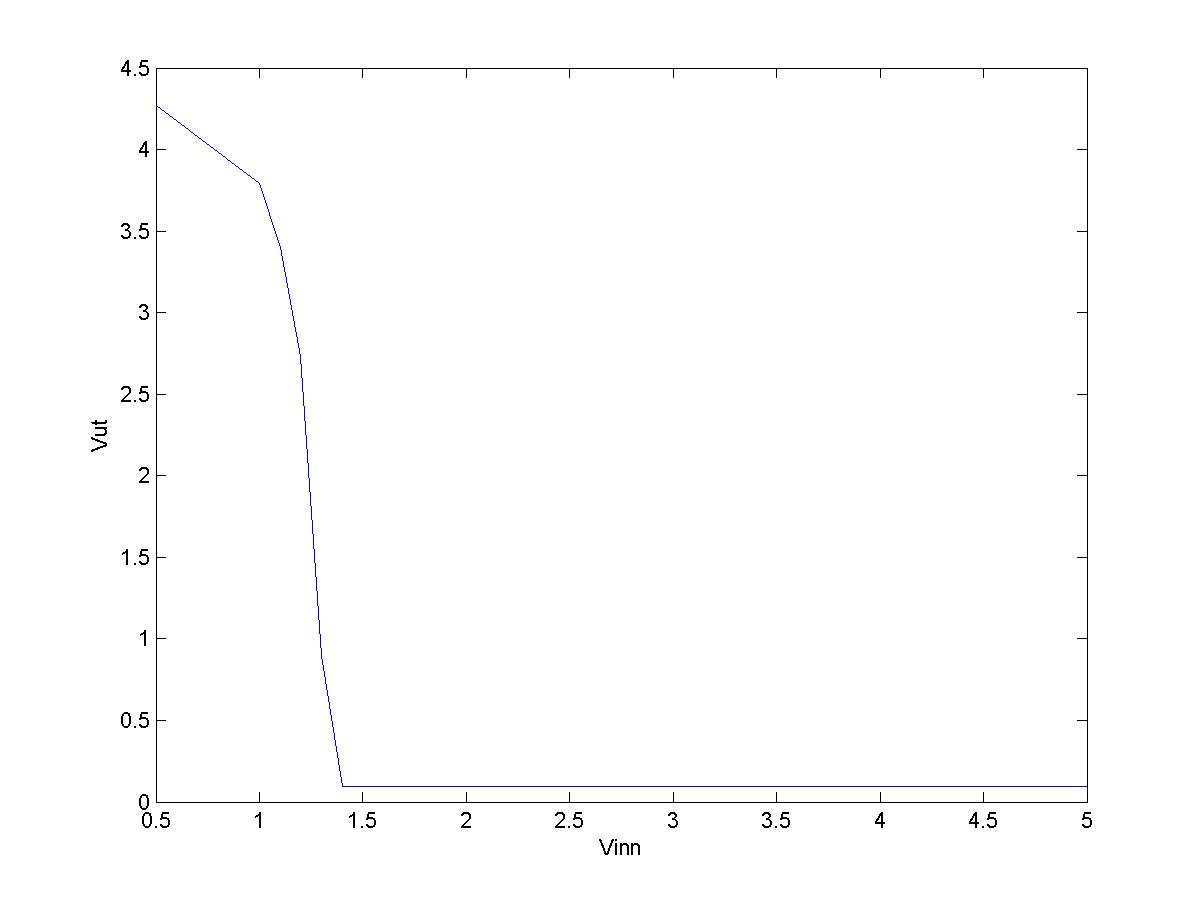
\includegraphics[width=\textwidth]{6a.jpg}
\end{figure}

Når vi skal måle strømmen er må vi regne ut spenningen over motstanden R5,
så vi kobler inn strap S3.
Vi måler spenningen over motstanden og regner ut strømmen basert på det, før vi
plotter det i forhold til inngangsmotstanden.

\begin{figure}[H]
  \caption{Forholdet mellom inngangstrøm og inngangsspenning.}
  \centering
    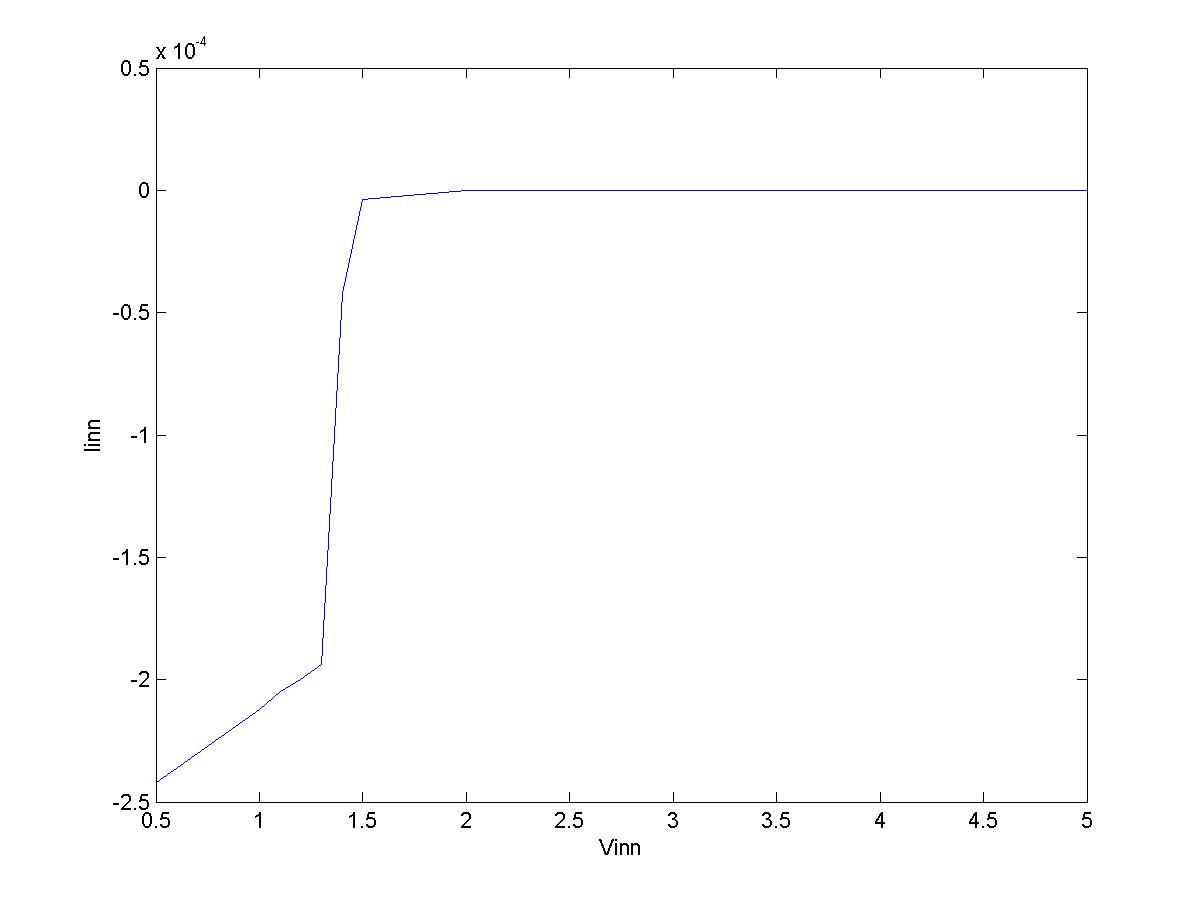
\includegraphics[width=\textwidth]{6aa.jpg}
\end{figure}



\subsection{Oppg 6a}
Vi setter frekvensen såpass høyt at vi ser utgangspulsens forsinkelse.
Når vi stiller inn cursor får vi en delta-tid på 33ns og en frekvens på 30MHz.
Det vil si at kretsen klarer å gjengi signaler på ~15MHz.
\begin{figure}[H]
  \caption{Forsinkelse i utgangspulsen.}
  \centering
    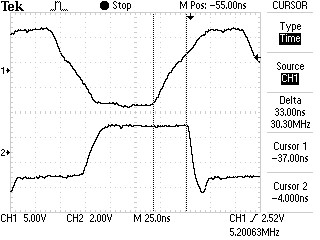
\includegraphics[width=\textwidth]{6b.jpg}
\end{figure}



\subsection{Oppg 6c}
TODO
